\section{Introduction}





As Large Language Model (LLM) agents engage in longer, open-ended interactions, they must handle growing histories that are essential yet challenging to leverage, motivating memory for retaining experience and maintaining coherence~\citep{hu2025memory}.
This need has driven rapid progress in agent memory, including approaches that summarize and retrieve past interactions or manage external memory stores~\citep{kang2025memory, chhikara2025mem0, packer2023memgpt, xu2025mem}. 
However, most methods still rely on static, hand-designed memory mechanisms, including fixed operation primitives (e.g., add/update/delete/skip)~\citep{wang2025mem, yan2025memory} and heuristic modules that govern what to store, how to revise it~\citep{kang2025memory, fang2025lightmem}, and when to prune it. Such designs bake in strong human assumptions and often suffer under diverse interaction patterns, scaling poorly as histories grow.




We argue that this formulation fundamentally limits the adaptability of agent memory.
Rather than treating memory as the output of fixed operations or hand-designed modules, we propose to elevate memory extraction itself into a \emph{learnable abstraction}.
Concretely, we view memory construction as the outcome of applying a small set of generic, reusable \emph{memory skills}: structured behaviors that specify when and how interaction traces should be transformed into memory and revised over time.
This perspective reveals a key bottleneck of prior pipelines: they hard-code memory behaviors into fixed procedural workflows that interleave heuristics with LLM-mediated extraction and revision, making them brittle under distribution shift~\citep{fang2025lightmem}.


Under this view, an ideal agent memory system should satisfy three properties.
(i) \textit{Minimal reliance on human priors.}
Instead of manually encoding what is worth remembering for a domain~\citep{zhong2024memorybank}, memory behaviors should be shaped by interaction data and updated as task demands evolve.
(ii) \textit{Support for larger extraction granularity.}
Many approaches are tuned to a fixed unit, such as per-turn processing~\citep{fang2025lightmem}, and can weaken when applied to longer spans.
A practical system should be able to operate at larger extraction granularity when needed.
(iii) \textit{Skill-conditioned, compositional memory construction.}
Existing systems often decompose memory construction into specialized modules~\citep{kang2025memory}.
In contrast, we prefer to \emph{select and compose} a small set of relevant skills for the current context and apply them in one generation step, enabling flexible reuse and evolution of memory behaviors.





\begin{figure*}[t]
	\centering
	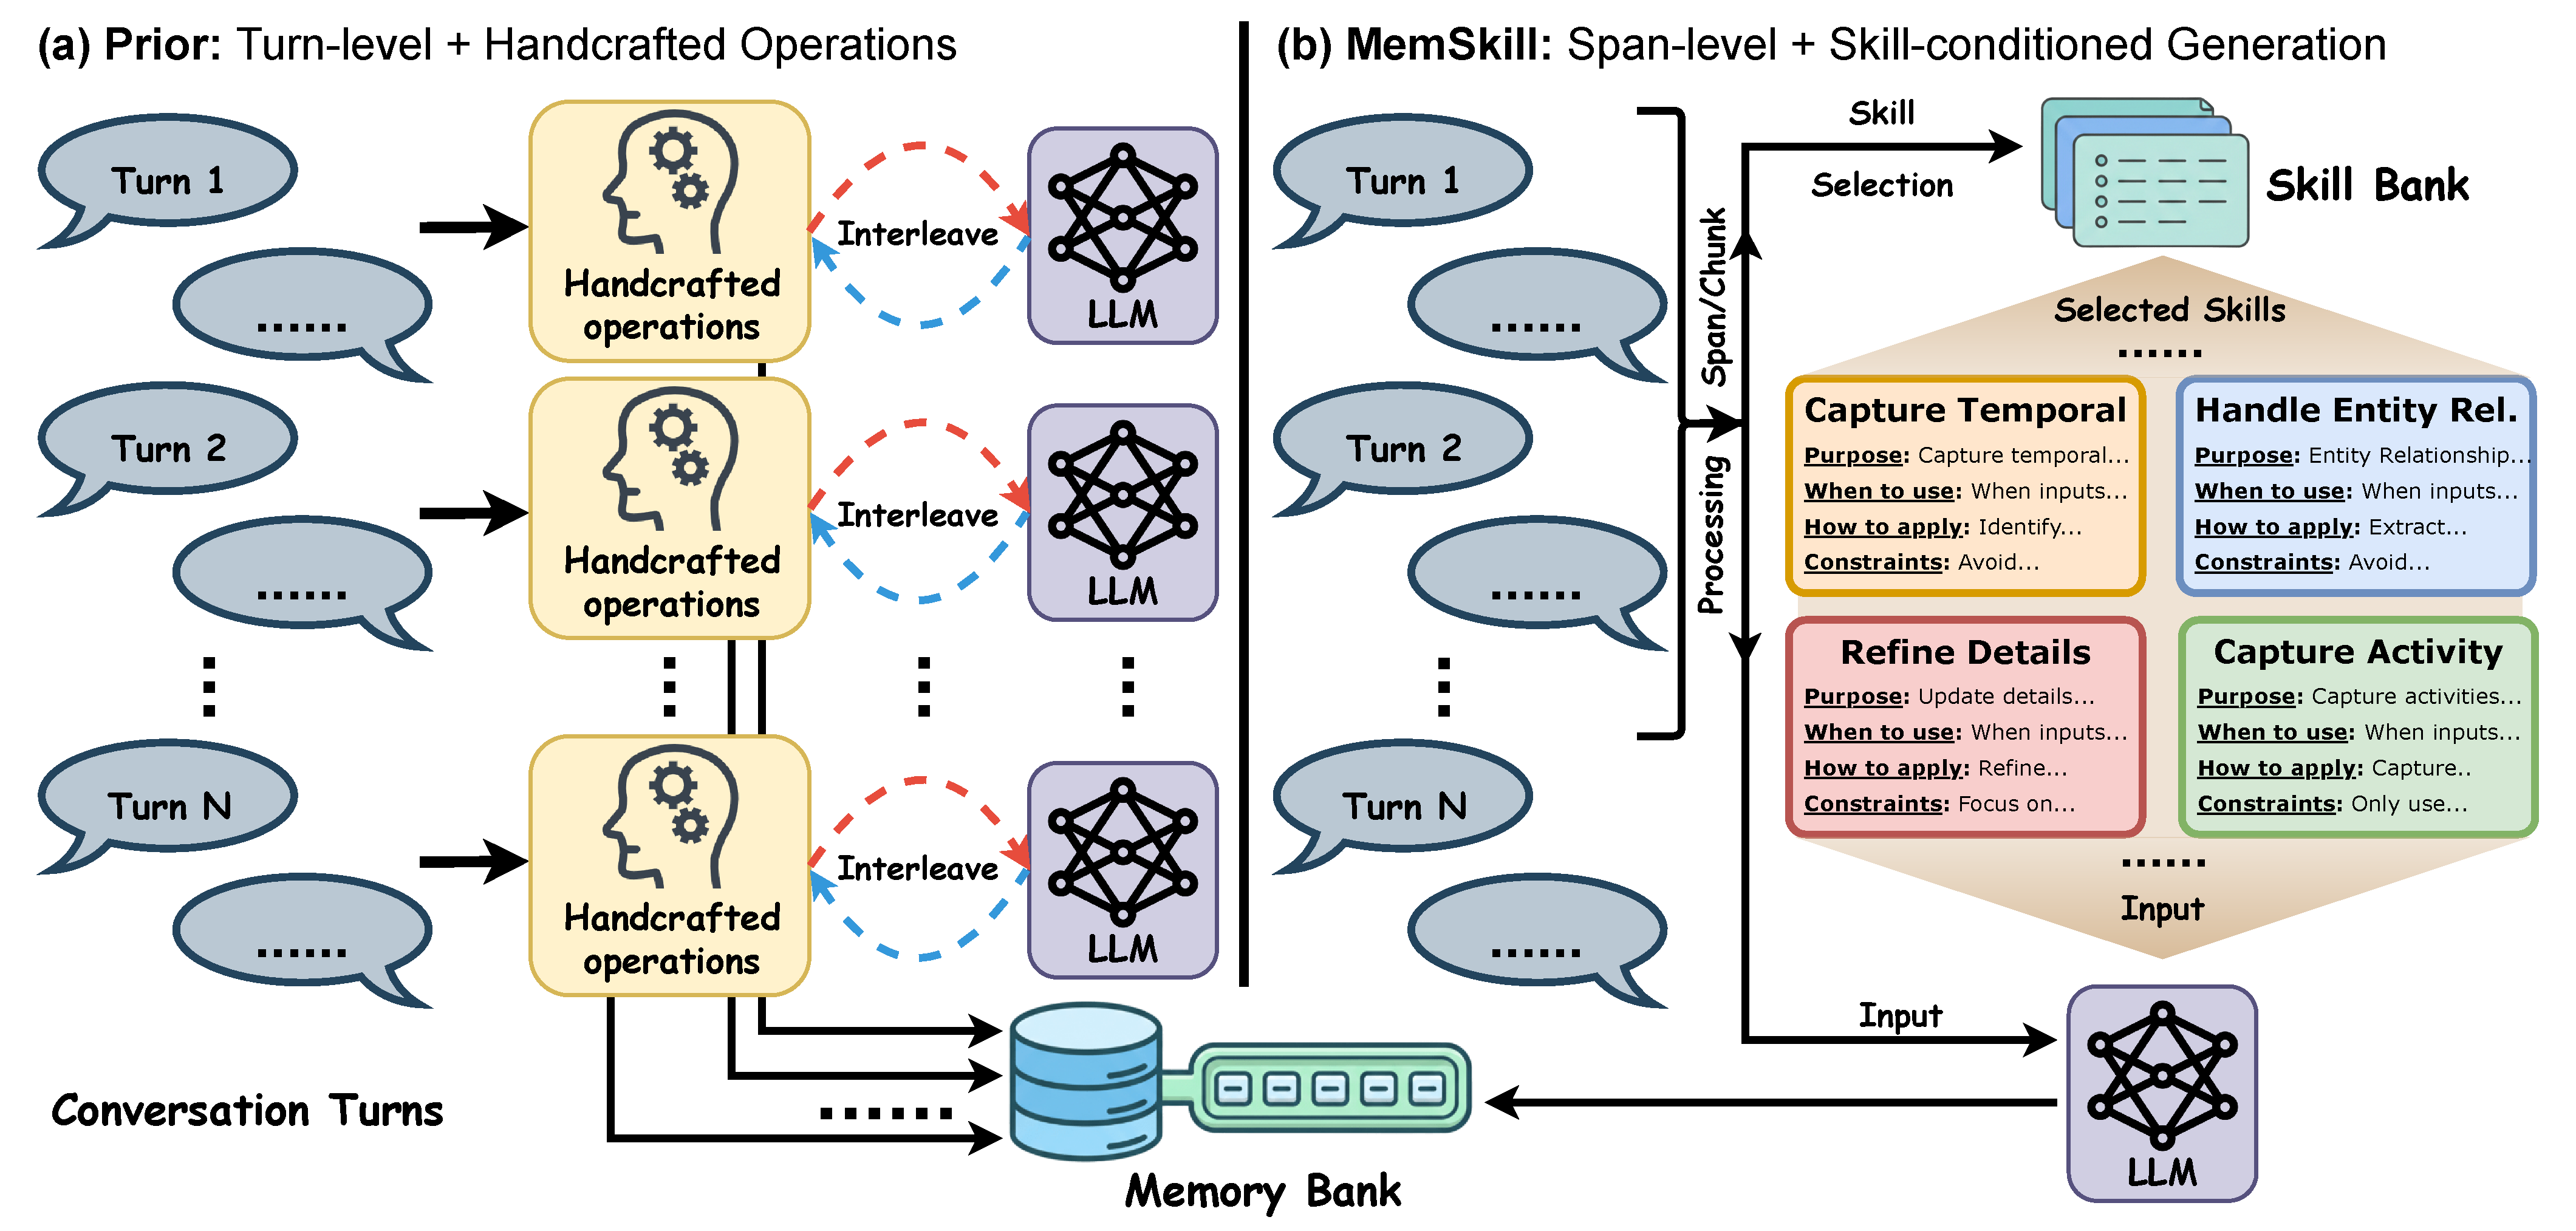
\includegraphics[width=1.0\linewidth]{figs/skill_intro.pdf}
        \caption{\textbf{Comparison between (a) prior turn-level, handcrafted operations and (b) MemSkill’s span-level, skill-conditioned generation.} Prior methods interleave handcrafted operations with LLM calls to incrementally extract and revise memory turn by turn, while MemSkill selects a small set of skills from a shared skill bank and applies them in one pass to produce skill-guided memories.}
	\label{intro_figure}
\end{figure*}




Based on the above observations, we introduce \textbf{MemSkill}, which reframes memory operations as a learnable and evolvable set of memory skills. 
MemSkill maintains a shared \emph{skill bank}, where each skill captures a reusable way to extract, consolidate, or revise memories from interaction text (Figure~\ref{intro_figure} shows the structured template of a memory skill). 
Given the current context, a \emph{controller} learns to select a small set of relevant skills, and an LLM-based \emph{executor} conditions on these skills to generate skill-guided memories in one pass.
This skill-conditioned formulation is not tied to a fixed extraction unit and can be applied to different span lengths when processing long interaction histories.


Crucially, MemSkill goes beyond learning how to use a fixed set of skills. We introduce a closed-loop evolution process that alternates between learning to use the current skill bank and evolving the skill bank itself. 
Specifically, we train the \emph{controller} with reinforcement learning (RL) using downstream task signals as feedback for skill selection. Periodically, a \emph{designer} aggregates the hardest cases produced during training, selects representative failures, and uses an LLM to refine existing skills and propose new ones. 
After each evolution step, the controller continues training on the evolved skill bank, with additional exploration to facilitate adopting newly introduced skills.
Overall, this process gradually strengthens both the skill selection policy and the evolving skill bank, moving toward a more adaptive memory management system driven by interaction data.


Experiments on LoCoMo, LongMemEval, HotpotQA, and ALFWorld show that MemSkill consistently improves task performance and generalizes well. Further analyses validate key components and showcase representative evolved skills, offering insights toward more adaptive, self-evolving memory management for LLM agents.



Our contributions can be summarized as follows.
\begin{itemize}
\item We propose \textbf{MemSkill}, an agent memory method that represents memory operations as an evolving skill bank, where each skill provides reusable guidance for selecting, extracting, and organizing useful memories. This turns memory construction from a fixed handcrafted pipeline into an adaptive skill-conditioned generation process.
\item We introduce a closed-loop optimization recipe that combines reinforcement learning for skill selection with LLM-guided skill evolution from hard cases, enabling continual refinement of the skill bank and taking a step toward self-evolving agent memory systems.
\item We evaluate MemSkill on LoCoMo, LongMemEval, HotpotQA, and ALFWorld, demonstrating consistent gains and strong transfer ability across conversational QA and embodied interaction settings, offering insights for self-evolving memory in LLM agents.
\end{itemize}





